\documentclass[12pt,a4paper,]{article}
\usepackage{amssymb,amsmath}
\newcommand*{\authorfont}{\fontfamily{phv}\selectfont}
\usepackage[]{libertine}


  \usepackage[T1]{fontenc}
  \usepackage[utf8]{inputenc}
\usepackage[scaled=0.9]{inconsolata}
% Uncomment the line below if you want to use XeLaTeX or 
% write on ShareLaTeX or Overleaf
% \setmonofont[Scale=0.90,BoldFont=inconsolata-bold.ttf]{inconsolata-regular.ttf}
\usepackage{color}
\definecolor{darkblue}{rgb}{0.0,0.0,0.55}
\usepackage{setspace}
\usepackage[top=2cm,bottom=2cm,left=2cm,right=2cm]{geometry}
\usepackage[backref,pagebackref]{hyperref}
\usepackage{graphicx}
\usepackage{float}
\usepackage{pgf}
\usepackage{tikz}
\usetikzlibrary{arrows}
\usetikzlibrary{positioning}
\usepackage{mathtools}
\usepackage{caption}
\usepackage[UKenglish]{babel}
\usepackage[UKenglish]{isodate}
\cleanlookdateon
\usepackage{babelbib} 
\exhyphenpenalty=1000
\hyphenpenalty=1000
\widowpenalty=1000
\clubpenalty=1000
\renewcommand*{\backref}[1]{}
\renewcommand*{\backrefalt}[4]{%
    \ifcase #1 (Not cited.)%
    \or        Cited on page~#2.%
    \else      Cited on pages~#2.%
    \fi}
\renewcommand{\backreftwosep}{ and~} 
\renewcommand{\backreflastsep}{ and~}
\hypersetup{
  linkcolor=darkblue,
  citecolor=darkblue,
  urlcolor=darkblue, 
  breaklinks=true, 
  colorlinks=true}
\doublespacing
\setlength{\parindent}{1cm}
\usepackage{ifxetex,ifluatex}
\usepackage{fixltx2e} % provides \textsubscript
\ifnum 0\ifxetex 1\fi\ifluatex 1\fi=0 % if pdftex
  \usepackage[T1]{fontenc}
  \usepackage[utf8]{inputenc}
\else % if luatex or xelatex
  \ifxetex
    \usepackage{amssymb,amsmath}
    \usepackage{mathspec}
  \else
    \usepackage{fontspec}
  \fi
  \defaultfontfeatures{Ligatures=TeX,Scale=MatchLowercase}
\fi
% use upquote if available, for straight quotes in verbatim environments
\IfFileExists{upquote.sty}{\usepackage{upquote}}{}
% use microtype if available
\IfFileExists{microtype.sty}{%
\usepackage{microtype}
\UseMicrotypeSet[protrusion]{basicmath} % disable protrusion for tt fonts
}{}
\hypersetup{unicode=true,
            pdftitle={Long Article Title: A Very Long Subtitle},
            pdfauthor={Your Name},
            pdfkeywords={R Markdown, pandoc, template},
            pdfborder={0 0 0},
            breaklinks=true}
\urlstyle{same}  % don't use monospace font for urls
\usepackage{natbib}
\bibliographystyle{apalike}
\usepackage{color}
\usepackage{fancyvrb}
\newcommand{\VerbBar}{|}
\newcommand{\VERB}{\Verb[commandchars=\\\{\}]}
\DefineVerbatimEnvironment{Highlighting}{Verbatim}{commandchars=\\\{\}}
% Add ',fontsize=\small' for more characters per line
\usepackage{framed}
\definecolor{shadecolor}{RGB}{248,248,248}
\newenvironment{Shaded}{\begin{snugshade}}{\end{snugshade}}
\newcommand{\KeywordTok}[1]{\textcolor[rgb]{0.13,0.29,0.53}{\textbf{{#1}}}}
\newcommand{\DataTypeTok}[1]{\textcolor[rgb]{0.13,0.29,0.53}{{#1}}}
\newcommand{\DecValTok}[1]{\textcolor[rgb]{0.00,0.00,0.81}{{#1}}}
\newcommand{\BaseNTok}[1]{\textcolor[rgb]{0.00,0.00,0.81}{{#1}}}
\newcommand{\FloatTok}[1]{\textcolor[rgb]{0.00,0.00,0.81}{{#1}}}
\newcommand{\ConstantTok}[1]{\textcolor[rgb]{0.00,0.00,0.00}{{#1}}}
\newcommand{\CharTok}[1]{\textcolor[rgb]{0.31,0.60,0.02}{{#1}}}
\newcommand{\SpecialCharTok}[1]{\textcolor[rgb]{0.00,0.00,0.00}{{#1}}}
\newcommand{\StringTok}[1]{\textcolor[rgb]{0.31,0.60,0.02}{{#1}}}
\newcommand{\VerbatimStringTok}[1]{\textcolor[rgb]{0.31,0.60,0.02}{{#1}}}
\newcommand{\SpecialStringTok}[1]{\textcolor[rgb]{0.31,0.60,0.02}{{#1}}}
\newcommand{\ImportTok}[1]{{#1}}
\newcommand{\CommentTok}[1]{\textcolor[rgb]{0.56,0.35,0.01}{\textit{{#1}}}}
\newcommand{\DocumentationTok}[1]{\textcolor[rgb]{0.56,0.35,0.01}{\textbf{\textit{{#1}}}}}
\newcommand{\AnnotationTok}[1]{\textcolor[rgb]{0.56,0.35,0.01}{\textbf{\textit{{#1}}}}}
\newcommand{\CommentVarTok}[1]{\textcolor[rgb]{0.56,0.35,0.01}{\textbf{\textit{{#1}}}}}
\newcommand{\OtherTok}[1]{\textcolor[rgb]{0.56,0.35,0.01}{{#1}}}
\newcommand{\FunctionTok}[1]{\textcolor[rgb]{0.00,0.00,0.00}{{#1}}}
\newcommand{\VariableTok}[1]{\textcolor[rgb]{0.00,0.00,0.00}{{#1}}}
\newcommand{\ControlFlowTok}[1]{\textcolor[rgb]{0.13,0.29,0.53}{\textbf{{#1}}}}
\newcommand{\OperatorTok}[1]{\textcolor[rgb]{0.81,0.36,0.00}{\textbf{{#1}}}}
\newcommand{\BuiltInTok}[1]{{#1}}
\newcommand{\ExtensionTok}[1]{{#1}}
\newcommand{\PreprocessorTok}[1]{\textcolor[rgb]{0.56,0.35,0.01}{\textit{{#1}}}}
\newcommand{\AttributeTok}[1]{\textcolor[rgb]{0.77,0.63,0.00}{{#1}}}
\newcommand{\RegionMarkerTok}[1]{{#1}}
\newcommand{\InformationTok}[1]{\textcolor[rgb]{0.56,0.35,0.01}{\textbf{\textit{{#1}}}}}
\newcommand{\WarningTok}[1]{\textcolor[rgb]{0.56,0.35,0.01}{\textbf{\textit{{#1}}}}}
\newcommand{\AlertTok}[1]{\textcolor[rgb]{0.94,0.16,0.16}{{#1}}}
\newcommand{\ErrorTok}[1]{\textcolor[rgb]{0.64,0.00,0.00}{\textbf{{#1}}}}
\newcommand{\NormalTok}[1]{{#1}}
\usepackage{longtable,booktabs}
\usepackage{graphicx,grffile}
\makeatletter
\def\maxwidth{\ifdim\Gin@nat@width>\linewidth\linewidth\else\Gin@nat@width\fi}
\def\maxheight{\ifdim\Gin@nat@height>\textheight\textheight\else\Gin@nat@height\fi}
\makeatother
% Scale images if necessary, so that they will not overflow the page
% margins by default, and it is still possible to overwrite the defaults
% using explicit options in \includegraphics[width, height, ...]{}
\setkeys{Gin}{width=\maxwidth,height=\maxheight,keepaspectratio}
\usepackage[normalem]{ulem}
% avoid problems with \sout in headers with hyperref:
\pdfstringdefDisableCommands{\renewcommand{\sout}{}}
  \IfFileExists{parskip.sty}{%
 \usepackage{parskip}
 }{% else
 \setlength{\parindent}{0pt}
 \setlength{\parskip}{0pt}
 }
  \setlength{\emergencystretch}{3em}  % prevent overfull lines
 \providecommand{\tightlist}{%
   \setlength{\itemsep}{0pt}\setlength{\parskip}{0pt}}
\setcounter{secnumdepth}{5}
% % % Redefines (sub)paragraphs to behave more like sections
% \ifx\paragraph\undefined\else
% \let\oldparagraph\paragraph
% \renewcommand{\paragraph}[1]{\oldparagraph{#1}\mbox{}}
% \fi
% \ifx\subparagraph\undefined\else
% \let\oldsubparagraph\subparagraph
% \renewcommand{\subparagraph}[1]{\oldsubparagraph{#1}\mbox{}}
% \fi
% 
\doublespacing

\title{Long Article Title:\\
A Very Long Subtitle\thanks{PhD candidate, Department of X, University of ZZ. Email address:
\href{mailto:your@email.com}{\nolinkurl{your@email.com}}. I would like
to thank \ldots{} for their helpful comments and suggestions. The usual
disclaimer applies. All data, code and information required to replicate
this study are available at the following web address:
\url{https://github.com/danilofreire/rmarkdown-article-template}.}}
\author{Your Name}
\date{12 March 2017}

\begin{document}
\maketitle

\begin{abstract}
\noindent Lorem ipsum dolor sit amet, consectetur adipiscing elit. Curabitur vitae
blandit ligula. Phasellus quis elit venenatis, suscipit lacus sed,
pellentesque risus. Proin vitae sapien id enim ultrices pretium ac eget
risus. Curabitur eget elit feugiat, congue orci sit amet, porttitor
libero. Vestibulum volutpat mauris tellus. Proin accumsan, velit ut
feugiat pulvinar, augue urna iaculis magna, et iaculis mi nunc vitae
justo. Nulla enim dui, elementum sit amet pharetra quis, tempus vitae
nisl.
\vspace{.5cm}

\noindent \textbf{Keywords}: R Markdown, pandoc, template
\vspace{.25cm}

\noindent \textbf{JEL Classification Codes}: A00, B11, C22
\end{abstract}
\newpage

\section{\texorpdfstring{Introduction\label{intro}}{Introduction}}\label{introduction}

\setlength{\parindent}{1cm} \setlength{\parskip}{0pt}

This is section \ref{intro}. \emph{Italics}, \textbf{boldface},
\texttt{typewriter}. Pellentesque quam justo, commodo nec gravida quis,
rutrum et nibh. Donec ornare iaculis dolor vitae euismod. Sed congue
lectus lorem, vel suscipit enim porttitor et. Morbi suscipit ex a sapien
condimentum elementum. Duis interdum condimentum ornare. Vivamus sit
amet dolor ultricies lacus laoreet maximus. Etiam imperdiet nunc a
malesuada varius. Sed sem velit, maximus id tincidunt vel, pulvinar in
neque.\footnote{This is a footnote. A citation:
  \citet[pp.~10--15]{freire2014}. An
  \href{http://github.com/danilofreire}{internet link}.}

Aenean tortor lacus, pharetra vel posuere eget, gravida non lorem.
Phasellus eros ante, dapibus tincidunt nisl eget, iaculis fermentum
odio. Suspendisse vitae nunc ac mauris semper molestie. Donec aliquam
tellus eros, non interdum eros iaculis ut. Phasellus nisl dui, aliquam
ullamcorper ante non, hendrerit molestie risus. Lorem ipsum dolor sit
amet, consectetur adipiscing elit. Fusce accumsan libero a purus
sodales, eget vulputate orci pellentesque. Morbi sit amet tellus
suscipit, gravida quam eget, mollis tortor. Etiam eu urna dictum,
condimentum nunc ut, ullamcorper elit. Table \ref{tab:tab1}:

\begin{longtable}[]{@{}lcr@{}}
\caption{Your Caption\label{tab:tab1}}\tabularnewline
\toprule
A & New & Table\tabularnewline
\midrule
\endfirsthead
\toprule
A & New & Table\tabularnewline
\midrule
\endhead
left-aligned & centre-aligned & right-aligned\tabularnewline
\$123 & \$456 & \$789\tabularnewline
\emph{italics} & \sout{strikethrough} & \textbf{boldface}\tabularnewline
\bottomrule
\end{longtable}

A \LaTeX \hspace{.005cm} equation:

\begin{equation}
Y = \beta_{0} + \beta_{1} X + \epsilon
\end{equation}

\begin{enumerate}
\def\labelenumi{\arabic{enumi}.}
\tightlist
\item
  Ordered
\item
  List

  \begin{enumerate}
  \def\labelenumii{\arabic{enumii}.}
  \tightlist
  \item
    Item
  \end{enumerate}
\end{enumerate}

\begin{itemize}
\tightlist
\item
  Unordered
\item
  List
\end{itemize}

\newpage

R chunk:

\begin{Shaded}
\begin{Highlighting}[]
\KeywordTok{data}\NormalTok{(}\StringTok{"mtcars"}\NormalTok{)}
\KeywordTok{summary}\NormalTok{(mtcars[, }\DecValTok{1}\NormalTok{:}\DecValTok{4}\NormalTok{])}
\end{Highlighting}
\end{Shaded}

\begin{verbatim}
##       mpg             cyl             disp             hp       
##  Min.   :10.40   Min.   :4.000   Min.   : 71.1   Min.   : 52.0  
##  1st Qu.:15.43   1st Qu.:4.000   1st Qu.:120.8   1st Qu.: 96.5  
##  Median :19.20   Median :6.000   Median :196.3   Median :123.0  
##  Mean   :20.09   Mean   :6.188   Mean   :230.7   Mean   :146.7  
##  3rd Qu.:22.80   3rd Qu.:8.000   3rd Qu.:326.0   3rd Qu.:180.0  
##  Max.   :33.90   Max.   :8.000   Max.   :472.0   Max.   :335.0
\end{verbatim}

\begin{Shaded}
\begin{Highlighting}[]
\KeywordTok{plot}\NormalTok{(mtcars$wt, mtcars$mpg, }\DataTypeTok{xlab =} \StringTok{"Car Weight"}\NormalTok{, }\DataTypeTok{ylab =} \StringTok{"Miles Per Gallon"}\NormalTok{, }
    \DataTypeTok{pch =} \DecValTok{19}\NormalTok{)}
\KeywordTok{abline}\NormalTok{(}\KeywordTok{lm}\NormalTok{(mpg ~}\StringTok{ }\NormalTok{wt, }\DataTypeTok{data =} \NormalTok{mtcars), }\DataTypeTok{col =} \StringTok{"red"}\NormalTok{)}
\end{Highlighting}
\end{Shaded}

\begin{figure}[htbp]
\centering
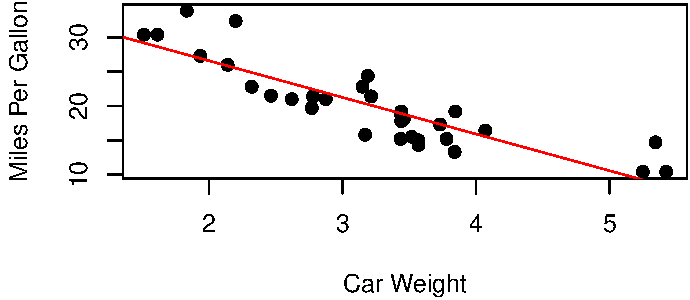
\includegraphics{article_files/figure-latex/unnamed-chunk-1-1.pdf}
\caption{A simple scatterplot with a caption quote}
\end{figure}

\newpage

\setlength{\parindent}{0cm} \setlength{\parskip}{6pt}

\bibliography{references.bib}

\end{document}
